% ################################################################
% If you separately execute this subfile, 
% the Chapter no, Page no, and Reference will always start at number 1.
%
% If you execute the thesis.tex, 
% the Chapter no, Page no, and Reference will be automatically and 
% continuously counted from previous chapters, 
% according to the order of files in thesis.tex.
% So, there is nothing to worry about numbering.
% ################################################################

\documentclass[../main/thesis.tex]{subfiles}

\begin{document}

\chapter{Existing Encoding Bitmap Indexes}
\label{ch:1}

The encoding strategy is regarded as being one of the preferable strategies for improving bitmap index if the small numbers of bitmap vectors are generated and these bitmap vectors are primarily used in the bitwise operations to precisely answer queries without any decompression and additional processing. This chapter describes the existing encoding bitmap indexes, including Range bitmap index, Interval bitmap index, Encoded bitmap index, Scatter bitmap index, and Dual bitmap index.

\section{Range bitmap index}
Let $C$ be the attribute cardinality, which is the number of distinct values of that indexed attribute. The Range bitmap index formed on the range encoding scheme \cite{RangeBI} produces a set of $C-1$ bitmap vectors, says $R$ = $\{R^0$, $R^1$, $\dots$, $R^{C-2}\}$. The attribute values represented by bitmap vector $R^j$ are ranging from 0 to $j$. The encoding function for this bitmap index, for attribute value $v$, is given in Eq. \eqref{eq:rangebi_encoding}

\begin{equation}
\label{eq:rangebi_encoding}
R^j=
\begin{cases}
1 & v \leq j \leq C-2 \\
0 & \text{Otherwise}.
\end{cases}
\end{equation}


\begin{figure}[!ht]
	\centering
	\subfloat[Table $T$]{
		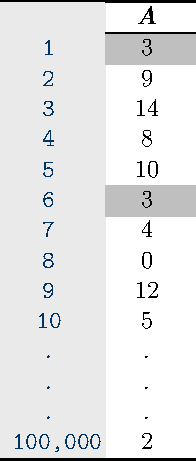
\includegraphics[scale=0.8, keepaspectratio]{table_t}
		\label{fig:table_t_range}}
	\hfil
	\subfloat[Range bitmap index]{
		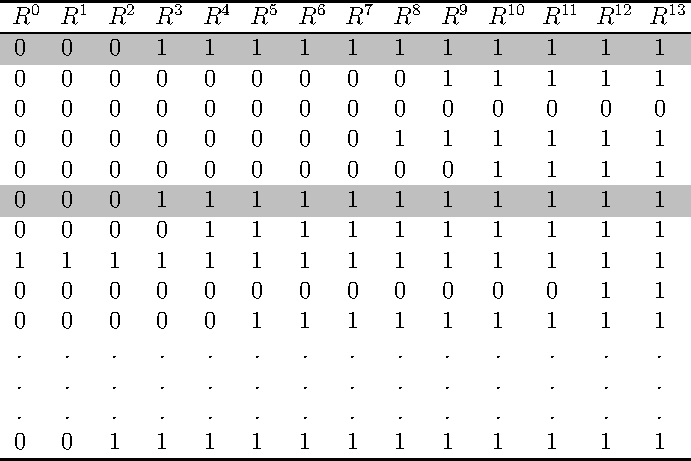
\includegraphics[scale=0.8, keepaspectratio]{table_range}
		\label{fig:table_range}}
	\caption{An example of the Range bitmap index: encoding of attribute $A$ with $C=15$.}
	\label{fig:example_range}
\end{figure}

Assume a domain of attribute $A$ given by table $T$ is $\{0$, $1$, $2$, $\dots$, $14\}$, as shown in Figure \subref*{fig:table_t_range}. The Range bitmap index therefore consists of 14 bitmap vectors since the cardinality of attribute $A$ is 15, says $\{R^0$, $R^1$, $R^2$, $\dots$, $R^{13}\}$. Using Eq. \eqref{eq:rangebi_encoding} to represent attribute value `3', all bits from $R^3$ to $R^{13}$ are set to bit value 1; otherwise, the bits remained are set to bit value 0, and these are highlighted in Figure \subref*{fig:table_range}.

Querying both equality and range on the Range bitmap index uses the retrieval function in Eq. \eqref{eq:rangebi_query}. Clearly, the equality queries deploy the first three conditions in Eq. \eqref{eq:rangebi_query}, and the range queries therefore deploy the remaining conditions.
\\
For $0 \leq v_1 < v_2 \leq C-1$,
\begin{equation}
\label{eq:rangebi_query}
v_1 \leq A \leq v_2 =
\begin{cases}
R^0 & v_1 = v_2 = 0, \\
R^{v_1} \oplus R^{v_1-1} & 0 < v_1 = v_2 < C-1 \\
\overline{R^{C-2}} & v_1 = v_2 = C-1 \\
\overline{R^{v_1-1}} & 0 < v_1 < C-1, v_2 = C-1 \\
R^{v_2} & v_1=0, 0 \leq v_2 \leq C-1 \\
R^{v_2} \oplus R^{v_1-1} & \text{Otherwise}.
\end{cases}
\end{equation}

For example, to evaluate the equality query in the form of $A=3$, using Eq. \eqref{eq:rangebi_query}, the bitmap vector $R^2$ and $R^3$ were scanned, and then the bitwise-XOR operator is performed on them to answer this equality query, yields $R^2 \oplus R^3$. This query results the \engordnumber{1} and \engordnumber{6} rows. 

To evaluate range query $1\leq A \leq 4$, using Eq. \eqref{eq:rangebi_query}, the bitmap vector $R^0$ and $R^4$ were scanned, and then the bitwise-XOR operator is performed on them to answer this range query, yields $R^4 \oplus R^0$.

\begin{prosNcons}{Advantage}
	The Range bitmap index offers a good query performance for equality and range queries with low cardinality. Sometimes, the Range bitmap index scans only one bitmap vector to answer equality queries if the query value is equal to 0 or $C-1$.
\end{prosNcons}

\begin{prosNcons}{Limitations}
	The Range bitmap index decreases one bitmap vector from the Basic bitmap index, which still suffered storage problem with high cardinality attributes. The query performance of Range bitmap index is degraded with high cardinality attributes for both equality and range queries in point of views space and time trade-off.
\end{prosNcons}

\begin{figure*}[!b]
	\centering
	\subfloat[Table $T$]{
		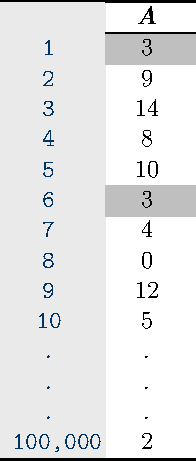
\includegraphics[scale=0.8, keepaspectratio]{table_t}
		\label{fig:table_t_interval}
	}
	\hfil
	\subfloat[Interval bitmap index]{
		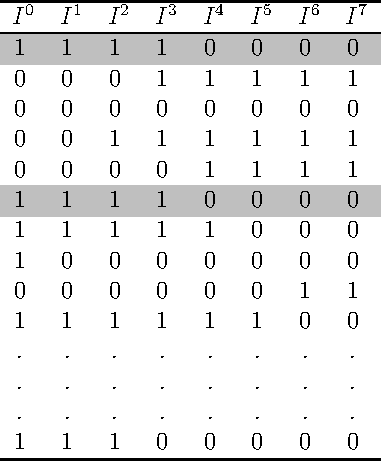
\includegraphics[scale=0.8, keepaspectratio]{table_interval}
		\label{fig:table_interval}
	}
	\caption{An example of the Interval bitmap index: encoding of attribute $A$ with $C=15$.}
	\label{fig:example_interval}
\end{figure*}

\section{Interval bitmap index}
The Interval bitmap index based on the interval encoding scheme \cite{IntervalBI} reduces the number of bitmap vectors by half to $\{I^0$, $I^1$, $\dots$, $I^{\lceil\frac{C}{2}\rceil -1}\}$. Each bitmap vector $I^j$ represents the range of values between $j$ and $j + m$, where $m = \lfloor\frac{C}{2}\rfloor -1$. The encoding function for the Interval bitmap index can be written as in Eq. \eqref{eq:intervalbi_encoding}. Figure \ref{fig:example_interval} shows as an example of the Interval bitmap index for the data in Figure \subref*{fig:table_t_interval}, with the 8 bitmap vectors, $\{I^0$, $I^1$, $\dots$, $I^7\}$. On encoding attribute value `3', all bits between $I^0$ and $I^3$ are set to 1 and the remaining bits are set to 0.

\begin{equation}
\label{eq:intervalbi_encoding}
I^j=
\begin{cases}
1 & v \leq j \leq j+m \\
0 & \text{Otherwise}.
\end{cases}
\end{equation}

The retrieval functions in Eq. \eqref{eq:intervalbi_query_equality} -- \eqref{eq:intervalbi_query_twoside} checks for equality, one-side range, and two-side range queries, respectively.

For example, to evaluate the equality query in the form of $A=3$, then the retrieval function of this query is $I^3 \wedge \overline{I^4}$. To evaluate range query in the form of $1\leq A \leq 4$, the bitmap vector $I^1$ and $I^5$ were scanned, and then the bitwise-OR operator is performed on them, yields $I^1 \wedge \overline{I^5}$.

\begin{equation}
\label{eq:intervalbi_query_equality}
A=v= 
\begin{cases}
I^0 & v=0,m=0 \\
\overline{I^0} & v=1,C=2 \\
I^1 & v=1,C=3 \\
I^v \wedge \overline{I^{v+1}} & v<m \\
I^1 \wedge I^0 & v=m,m>0 \\
I^{v-m} \wedge \overline{I^{v-m-1}} & m<v<C-1,m>0 \\
\overline{I^{ \left\lceil \frac{C}{2} \right\rceil -1} \vee I^0} & v=C-1.
\end{cases}
\end{equation}
\\
For $0<v<C-1$,
\begin{equation}
\label{eq:intervalbi_query_oneside}
A\leq v = 
\begin{cases}
I^0 \wedge \overline{I^{v+1}} & v < m \\
I^0 & v=m \\
I^0 \vee I^{v-m} & m < v < C-1.
\end{cases}
\end{equation}
\\
For $0<v_1<v_2<C-1$,
\begin{equation}
\label{eq:intervalbi_query_twoside}
v_1 \leq A \leq v_2 = 
\begin{cases}
I^{v_1} \wedge \overline{I^{v_2}+1} & v_2<m \\
I^{v_1} \wedge I^0 & v_2=m \\
I^{v_1} \wedge I^{v_2-m} & v_2<v_1+m,v_1<n \\
I^{v_1} & v_2=v_1+m,v_1<n \\
I^{v_1} \vee I^{v_2-m} & v_2>v_1+m,v_1<m \\
I^{v_1} \vee I^{v_1+1} & v_2=v_1+m+1,v_1=m \\
I^{v_2-m} \wedge \overline{I^{v_1-m-1}} & v_1 \geq n.
\end{cases}
\end{equation}

\begin{prosNcons}{Advantage}
	The index size used by the Interval bitmap index is much smaller than that used by the Basic and Range bitmap index. In addition, the Interval bitmap index offers improved query performance against the Range bitmap index for both equality and range queries with low cardinality.
\end{prosNcons}

\begin{prosNcons}{Limitations}
	The Interval bitmap index still produces many bitmap vectors with high cardinality, which is an impact on storage requirement. The performance of Interval bitmap index is degraded with high cardinality attributes for both equality and range queries in point of views space and time trade-off.
\end{prosNcons}

\section{Encoded bitmap index}
To our knowledge, the Encoded bitmap index \cite{EncodedBI} produces the smallest number of bitmap vectors, which consists of $\lceil\log_2 C\rceil$ bitmap vectors, say $\{E^0$, $E^1$, $\dots$, $E^{\lceil\log_2 C\rceil -1}\}$, and a mapping table which stores the binary patterns of all distinct attribute values. The attribute values are encoded with $\lceil\log_2 C\rceil$ bits in corresponding position of the bitmap vectors. Figure \ref{fig:example_encoded} shows an example of the Encoded bitmap index for the attribute with cardinality 15, which consists of 4 bitmap vectors, $E^0$, $E^1$, $E^2,$ and $E^3$. Let us consider encoding the attribute value `3'. The binary pattern for attribute value `3' in the mapping table is `0011'. Therefore, the bitmap vectors are set, for this item, as $E^0 = 0$, $E^1 = 0$, $E^2 = 1$, and $E^3 = 1$, respectively.

\begin{figure*}[!t]
	\centering
	\subfloat[Table $T$]{
		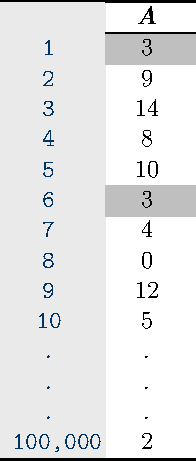
\includegraphics[scale=0.8, keepaspectratio]{table_t}
		\label{fig:table_t_encoded}
	}
	\hfil
	\subfloat[Encoded bitmap index with a mapping table]{
		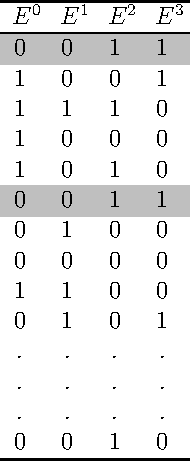
\includegraphics[scale=0.8, keepaspectratio]{table_encoded} \qquad \qquad
		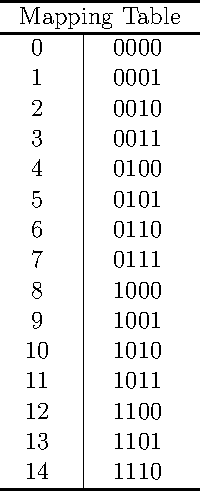
\includegraphics[scale=0.75, keepaspectratio]{table_encoded_mapping}
		\label{fig:table_encoded}
	}
	\caption{An example of the Encoded bitmap index: encoding of attribute $A$ with $C=15$.}
	\label{fig:example_encoded}
\end{figure*}

To evaluate equality queries, the binary pattern of the query value is retrieved from the mapping table, and then the $\lceil\log_2 C\rceil$ bitmap vectors are jointly checked for this pattern in each row. Rows matching the target pattern across the $\lceil\log_2 C\rceil$ bits are returned as the answer to the query. Unfortunately, the traditional equality query processing used by the Encoded bitmap index takes a long time to answer the query because of the comparison of all $\lceil\log_2 C\rceil$ bitmap vectors. Accordingly, the E-EBI \cite{EEBI} is introduced to improve the traditional equality query processing in the Encoded bitmap index without comparison all bitmap vectors. In this algorithm, the bitmap vector can be performed bitwise-AND operation directly if the corresponding bit is set to 1. Otherwise, the negation of the bitmap vector is required before performing bitwise-AND operation. For example, to evaluate the equality query $A=3$, the binary pattern for attribute value `3' is `0011', given by the mapping table in Figure \subref*{fig:table_encoded}.   Therefore, the negation of bitmap vector $E^0$ and $E^1$ is required before performing bitwise-AND operation. As a result, the retrieval function of this query is simply created as $\overline{E^0}\overline{E^1}E^2E^3$.

For evaluating range queries, the retrieval function for the query is formed of Boolean expressions that apply bitwise-OR operators on the expressions to get the final result. For example, to evaluate range query $1\leq A \leq 4$, the binary patterns for each item are retrieved from the mapping table, and transformed to Boolean expressions, yields $\overline{E^0}\overline{E^1}\overline{E^2}E^3$ for value 1, $\overline{E^0}\overline{E^1}E^2\overline{E^3}$ for value 2,
$\overline{E^0}\overline{E^1}E^2 E^3$ for value 3,
$\overline{E^0}E^1\overline{E^2}\overline{E^3}$ for value 4. Then, the bitwise-OR operators are used on them, yields $(\overline{E^0}\overline{E^1}\overline{E^2}E^3) \vee (\overline{E^0}\overline{E^1}E^2\overline{E^3}) \vee (\overline{E^0}\overline{E^1}E^2 E^3) \vee (\overline{E^0}E^1\overline{E^2}\overline{E^3})$. Furthermore, the generated retrieval function can be further reduced to optimize range query performance by utilizing Boolean minimization method, such as Quine-McCluskey algorithm \cite{Quine1952,Mccluskey1956}. The reduced retrieval function by Quine-McCluskey algorithm is generated as $(\overline{E^0}\overline{E^1} E^3) \vee (\overline{E^0}\overline{E^1}E^2\overline{E^3}) \vee (\overline{E^0}E^1\overline{E^2}\overline{E^3})$. Additionally, the improved algorithms for Encoded bitmap index were introduced for querying equality and range queries by using data mining techniques and parallel processing over large dataset \cite{ApioriEncoded, FIEncoded, EEBI, DistEQ}. However, both equality and range queries on the Encoded bitmap index take long execution times, even though this bitmap index is effective from the space requirement point of view.

\begin{prosNcons}{Advantage}
	The Encoded bitmap index requires the smallest number of bitmap vectors for all cardinalities, which is an efficiency in space requirement.
\end{prosNcons}

\begin{prosNcons}{Limitations}
	The query execution time taken by Encoded bitmap index is undesirable for both equality and range queries. Even though the Encoded bitmap index uses the Boolean minimization method in range queries to reduce the complexity of the retrieval function, it considerably takes long processing times with range queries.
\end{prosNcons}


\section{Scatter bitmap index}
For Scatter bitmap index \cite{ScatterBI}, the bitmap vectors are split into two groups, namely Z-group and L-group. The Scatter bitmap index uses $\lceil 2\sqrt{C}\rceil$ bitmap vectors. The Z-group contains $\lceil\frac{C}{m-1}\rceil + 1$ bitmap vectors, says $\{Z^0$, $Z^1$, $\dots$, $Z^{\lceil\frac{C}{m-1}\rceil}\}$, while the L-group contains $m-2$ bitmap vectors, say $\{L^1$, $L^2$, $\dots$, $L^{m-2}\}$, where $m = \lceil\sqrt{C} \rceil + 1$.

\begin{algorithm}[ht]
	\caption{The creation of Scatter bitmap index}
	\label{alg:scatter_create_algorithm}
	\begin{algorithmic}[1]
		\INPUT{The cardinality and values of of the indexed attribute}
		\OUTPUT{The scatter bitmap index}
		\State $m \gets \lceil\sqrt{C}\rceil + 1$
		\FOR{a value $'v' $ in each row} 
		\State Initial all bits in the bitmap vectors of Z- and L-group to be 0
		\State $j \gets \lfloor \frac{v}{m-1} \rfloor +1$ 
		\State $k \gets v \mod m-1$
		\If{$k = 0$}
		\State Set bit of $Z^{j-1}$ and $Z^j$ to be 1
		\Else
		\State Set bit of $L^k$ and $Z^j$ to be 1
		\EndIf
		\ENDFOR
	\end{algorithmic}
\end{algorithm}

The algorithm for creation Scatter bitmap index is shown in Algorithm \ref{alg:scatter_create_algorithm}. If the value `$v$' at i\textsuperscript{th} row relates to $Z^{j-1}$ and $Z^j$ (or $L^k$ and $Z^j$), the bits in $Z^{j-1}$ and $Z^j$ (or $L^k$ and $Z^j$) at i\textsuperscript{th} row are set to 1. Otherwise, they are set to 0. Figure \ref{fig:example_scatter} depicts an example of Scatter bitmap index for an attribute of cardinality 15, which consists of 8 bitmap vectors, say $\{Z^0$, $Z^1$, $Z^2$, $Z^3$, $Z^4$, $L^1$, $L^2$, $L^3\}$, and $m=5$. On encoding attribute value `3', the bits in $Z^1$ and $L^3$ are set to 1 and the remaining bits are set to 0, due to the values of $j$ and $k$ are 1 and 3, respective, corresponding to the \engordnumber{2} and \engordnumber{11} steps in Algorithm \ref{alg:scatter_create_algorithm}. Then, the bits in $Z^1$ and $L^3$ are set to 1 and the remaining bits are set to 0.

\begin{figure}[ht]
	\centering
	\subfloat[Table $T$]{
		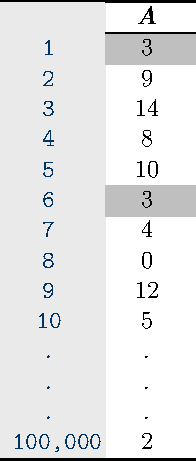
\includegraphics[scale=0.8, keepaspectratio]{table_t}
		\label{fig:table_t_scatter}
	}
	\hfil
	\subfloat[Scatter bitmap index]{
		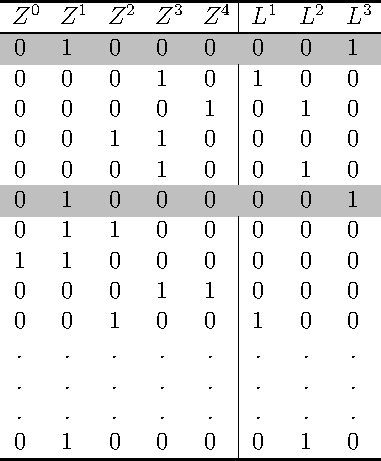
\includegraphics[scale=0.8, keepaspectratio]{table_scatter}
		\label{fig:table_scatter}
	}
	\caption{An example of the Scatter bitmap index: encoding of attribute $A$ with $C=15$.}
	\label{fig:example_scatter}
\end{figure}


Equality queries with Scatter bitmap index use the retrieval function in Eq. \eqref{eq:scatterbi_retrieval}. For example, to answer the equality query $A=3$. Using Eq. \eqref{eq:scatterbi_retrieval}, the retrieval function of this query is $Z^1 \wedge L^3$.

\begin{equation}
\label{eq:scatterbi_retrieval}
A=v=
\begin{cases}
Z^{j-1} \wedge Z^j & k=0 \\
Z^j \wedge L^k & \text{Otherwise}.
\end{cases}
\end{equation}
\begin{conditions}
	$m$ & = & $\left\lceil \sqrt{C} \right\rceil +1$\\
	$j$ & = & $\left\lfloor \frac{v}{m-1} \right\rfloor +1$ \\
	$k$ & = & $v \text{ mod } (m-1)$
\end{conditions}

For evaluating range queries, two bitmap vectors associated with each query value can be dynamically created by using Eq. \eqref{eq:scatterbi_retrieval}, and the retrieval is performed with bitwise-OR operations. For example, to answer the range query $1 \leq A \leq 4$, by using Eq. \eqref{eq:scatterbi_retrieval}, the retrieval functions for representing each item are dynamically generated as $Z^1 \wedge L^1$ for value 1, $Z^1 \wedge L^2$ for value 2, $Z^1 \wedge L^1$ for value 3, $Z^1 \wedge Z^2$ for value 4. Then, the bitwise-OR operators are used on them, yields $(Z^1 \wedge L^1) \vee (Z^1 \wedge L^2) \vee (Z^1 \wedge L^2) \vee (Z^1 \wedge Z^2)$. Furthermore, the retrieval function can be further minimized, which impacts the numbers of bitmap vectors accessed and the numbers of Boolean operations used. The basis idea of Dual-simRQ \cite{Keawpibal2018Dual} is modified and applied to improve query processing, especially range queries. Therefore, the final reduced retrieval function is generated as $\left(Z^1 \wedge (L^1 \vee L^2 \vee L^3)\right) \vee (Z^1 \wedge Z^2)$. Additionally, the data clustering technique was employed to optimize the query processing on the Scatter bitmap index by grouping the attribute values which is frequently queried \cite{Weahama2009}, to improve query execution time used by Scatter bitmap index.  

\begin{prosNcons}{Advantage}
	The Scatter bitmap index requires the less space than the Basic, Range, and Interval bitmap indexes, except the Encoded bitmap index. The Scatter bitmap index is suitable for equality queries because of scanning two bitmap vectors.
\end{prosNcons}

\begin{prosNcons}{Limitations}
	The query execution time used by Scatter bitmap index is slower than the Basic bitmap index for equality queries. For range queries, the query execution time used by Scatter bitmap index is undesirable. Therefore, the performance of Scatter bitmap index with range queries is poor in space vs. time trade-off point of view.
\end{prosNcons}

\section{Dual bitmap index}
In the Scatter bitmap index, one bitmap vector (i.e., $Z^0$) is used to represent one value, which wastes space. Improving the Scatter bitmap index, the Dual bitmap index \cite{DualBI} efficiently represents attribute values while using two bitmap vectors. The Dual bitmap index consists of $\lceil\sqrt{2C+0.25}+0.5 \rceil$  bitmap vectors, say $\{D^0$, $D^1$, $\dots$, $D^{\lceil\sqrt{2C+0.25}+0.5 \rceil -1}\}$. The dual encoding function is given in Eq. \eqref{eq:dualbi_encoding}.

\begin{equation}
\label{eq:dualbi_encoding}
D^j=
\begin{cases}
1 & j=r \text{ and } j=s \\
0 & \text{Otherwise}.
\end{cases} 
\end{equation}
\begin{conditions}
	$hiC$ & = & $\frac{n(n-1)}{2}$\\
	$r$   & = & $\left\lceil \sqrt{2(hiC-v)+0.25}+0.5 \right\rceil$ \\
	$s$   & = & $\left\lceil r-1- \left[ \left( v- \frac{(n-r)(n-r-1)}{2} \right ) \text{ mod } r \right] \right\rceil$
\end{conditions}

Figure \ref{fig:example_dual} depicts an example of the Dual bitmap index for an attribute with cardinality 15, with 6 bitmap vectors, say $\{D^0$, $D^1$, $D^2$, $D^3$, $D^4$, $D^5\}$. Using Eq. \eqref{eq:dualbi_encoding}, to represent attribute value `3', the bits in $D^1$ and $D^5$ are set to 1, while the remaining bits are set to 0. 

\begin{figure}[ht]
	\centering
	\subfloat[Table $T$]{
		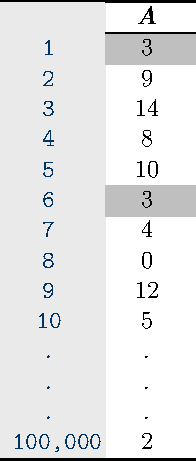
\includegraphics[scale=0.8, keepaspectratio]{table_t}
		\label{fig:table_t_dual}
	}
	\hfil
	\subfloat[Dual bitmap index]{
		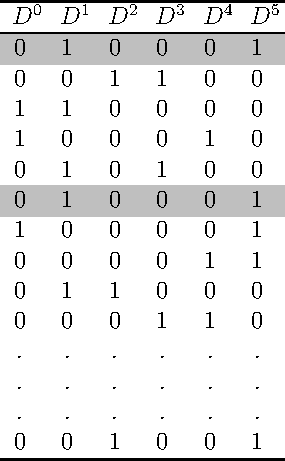
\includegraphics[scale=0.8, keepaspectratio]{table_dual}
		\label{fig:table_dual}
	}
	\caption{An example of the Dual bitmap index: encoding of attribute $A$ with $C=15$.}
	\label{fig:example_dual}
\end{figure}

Evaluation of equality queries with the Dual bitmap index uses the retrieval function in Eq. \eqref{eq:dualbi_retrieval}. For example, to answer the equality query $A=3$. Using Eq. \eqref{eq:dualbi_retrieval}, the retrieval function of this query is $D^5 \wedge D^1$.

\begin{equation}
\label{eq:dualbi_retrieval}
A=v=D^r \wedge D^s
\end{equation}

To answer range queries, the retrieval function can be dynamically created and performed bitwise-OR operators, similar to the case with Scatter bitmap index. For example, to answer the range query $1 \leq A \leq 4$, by using Eq. \eqref{eq:dualbi_retrieval}, the retrieval functions for representing each item are dynamically generated as $D^5 \wedge D^3$ for value 1, $D^5 \wedge D^2$ for value 2, $D^5 \wedge D^1$ for value 3, $D^5 \wedge D^0$ for value 4. Then, the bitwise-OR operators are used on them, yields $(D^5 \wedge D^3) \vee (D^5 \wedge D^2) \vee (D^5 \wedge D^1) \vee (D^5 \wedge D^0)$. In addition, the retrieval function can be minimized to reduce the scanning of bitmap vectors as well as the number of Boolean operations, which impacts the query execution time taken. Therefore, Dual-simRQ \cite{Keawpibal2018Dual} was proposed to improve the query execution time with range queries. The reduced retrieval function generated by Dual-simRQ is $D^5 \wedge (D^3 \vee D^2 \vee D^1 \vee D^0)$.

\begin{prosNcons}{Advantage}
	The Dual bitmap index requires the less space than the Basic, Range, Interval, and Scatter bitmap indexes, except the Encoded bitmap index. The performance of Dual bitmap index is better than the existing bitmap indexes in terms of space and time trade-off for equality queries.
\end{prosNcons}

\begin{prosNcons}{Limitations}
	The query execution time used by Dual bitmap index is slower than the Basic bitmap index for equality queries. Furthermore, the query execution time with range queries used by Dual bitmap index is undesirable. Therefore, the performance of Dual bitmap index is degraded in space vs. time trade-off for range queries.
\end{prosNcons}

The numbers of bitmap vectors used for encoding bitmap indexes are summarized in Table \ref{tab:sumarize_bitmapvector}. The Basic bitmap index uses $C$ bitmap vectors while the Range and Interval bitmap indexes decrease the number of bitmap vectors by one and half, respectively. The Encoded bitmap index uses $\left\lceil \log_2 C \right\rceil$ bitmap vectors. The Scatter and Dual bitmap indexes utilize $\lceil 2\sqrt{C}\rceil$ and $\lceil\sqrt{2C+0.25}+0.5 \rceil$ bitmap vectors, respectively.

\begin{table}[h]
	\setlength{\tabcolsep}{15pt}
	\centering
	\caption{A summarization of the number of bitmap vectors used for six encoding bitmap indexes}
	\label{tab:sumarize_bitmapvector}
	\begin{tabular}{l c}
		\toprule
		Bitmap index & The number of bitmap vectors used \\
		\midrule
		Basic & $C$ \\
		Range & $C-1$ \\
		Interval & $\left\lceil \frac{C}{2} \right\rceil$ \\
		Encoded & $\left\lceil \log_2 C \right\rceil$ \\
		Scatter & $\lceil 2\sqrt{C}\rceil$ \\
		Dual & $\lceil\sqrt{2C+0.25}+0.5 \rceil$ \\
		\bottomrule
	\end{tabular}
\end{table}

\begin{figure}[!b]
	\centering
	{\subfloat[Basic scheme]{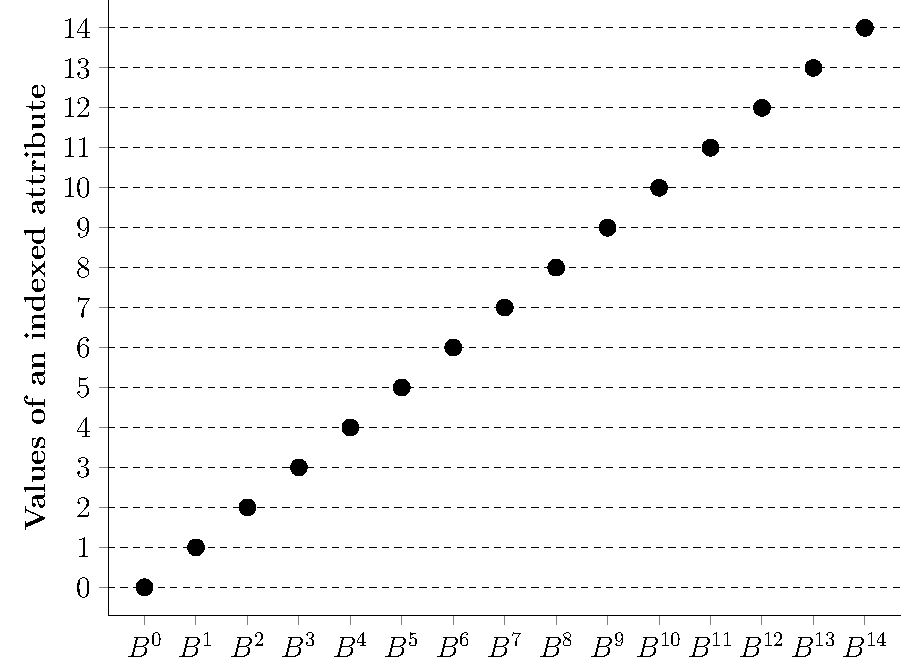
\includegraphics[scale=0.42]{encoding_basic}
			\label{fig:encoding_basic}}}
	\hfil
	{\subfloat[Range scheme]{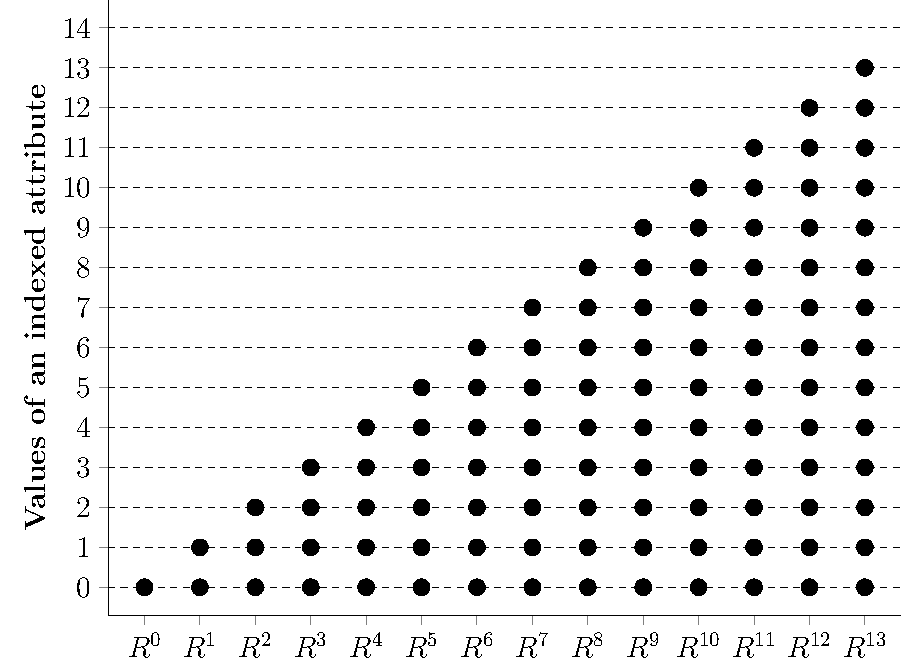
\includegraphics[scale=0.42]{encoding_range}
			\label{fig:encoding_range}}}
	\hfil
	{\subfloat[Interval scheme]{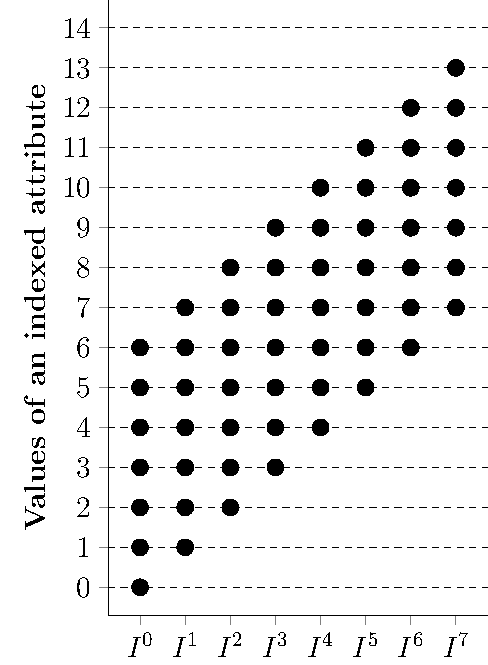
\includegraphics[scale=0.42]{encoding_interval}
			\label{fig:encoding_interval}}}
	\hfil
	{\subfloat[Encoded scheme]{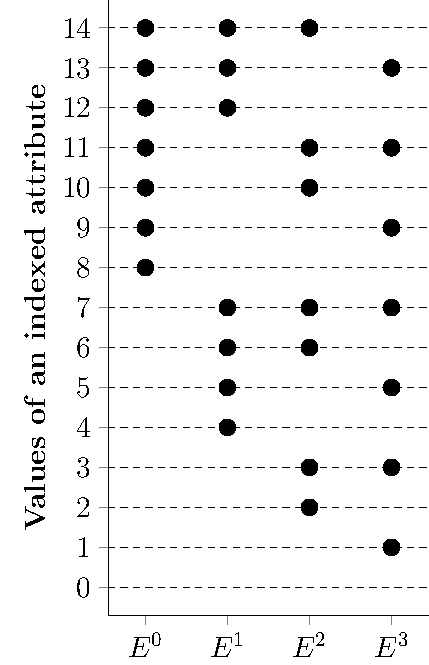
\includegraphics[scale=0.42]{encoding_encoded}
			\label{fig:encoding_encoded}}}
	\hfil
	{\subfloat[Scatter scheme]{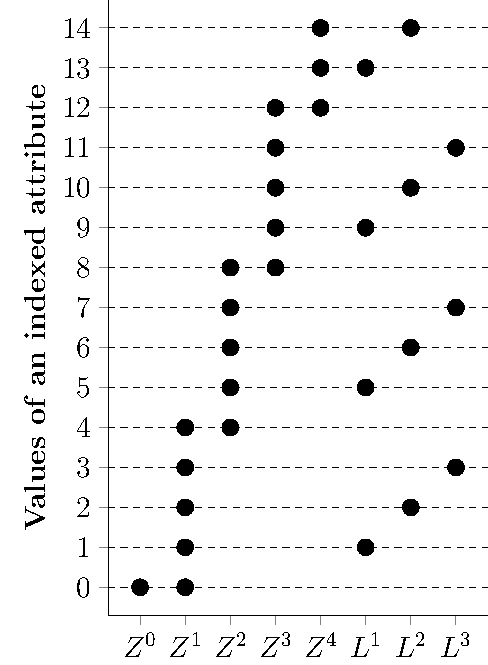
\includegraphics[scale=0.42]{encoding_scatter}
			\label{fig:encoding_scatter}}}
	\hfil
	{\subfloat[Dual scheme]{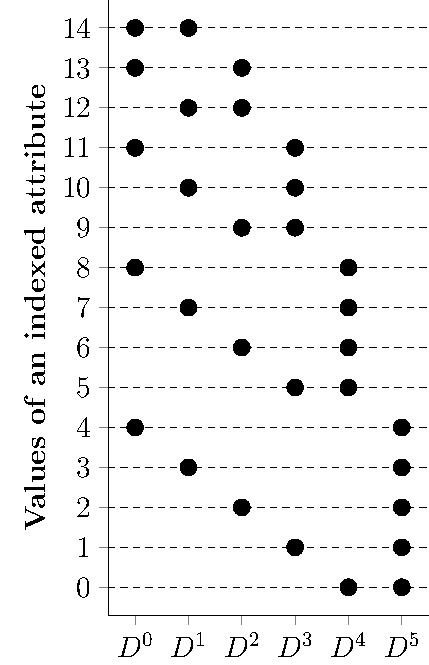
\includegraphics[scale=0.42]{encoding_dual}
			\label{fig:encoding_dual}}}
	\hfil
	\caption{Six encoding schemes with $C$ = 15, ($\bullet$ represents bit 1).}
	\label{fig:encoding_schemes}
\end{figure}

Figure \ref{fig:encoding_schemes} illustrates the six encoding schemes with $C= 15$. Note that the black dots denote bit value 1. The Basic bitmap index uses 15 bitmap vectors, shown in Figure \subref*{fig:encoding_basic}. The Range bitmap index uses 14 bitmap vectors while the Interval bitmap index uses 8 bitmap vectors to represent the attribute values, shown in Figure \subref*{fig:encoding_range} and \subref*{fig:encoding_interval}, respectively. The Encoded bitmap index uses 4 bitmap vectors, shown in Figure \subref*{fig:encoding_encoded}. Figures \subref*{fig:encoding_scatter} and \subref*{fig:encoding_dual} show the encoding schemes for the Scatter and Dual bitmap indexes, which use 8 and 6 bitmap vectors, respectively.

This chapter described the characteristics of five encoding bitmap indexes, including Range, Interval, Encoded, Scatter, and Dual bitmap indexes. The Range and Interval bitmap indexes are efficient for equality and range queries by setting bit value 1 in the consecutive bitmap vectors to represent attribute values. However, those bitmap indexes suffer from high storage requirements, due to the large numbers of bitmap vectors. While the Encoded bitmap index uses the smallest number of bitmap vectors, it is inefficient with equality and range queries. The Scatter and Dual bitmap indexes can improve the performance for equality query processing, in terms of space and time trade-off, by accessing two bitmap vectors. Unfortunately, the range query processing is unsatisfactory. Table \ref{tab:summary_encoding} summarizes the advantages and limitations of six encoding bitmap index algorithms.

As aforementioned, the existing encoding bitmap indexes are not be able to fully solve the problems of both space requirements and execution times with a variety of submitted queries. Therefore, the proposed encoding bitmap index, called HyBiX for Hybrid Encoding Bitmap Index, will be explained in the next chapter, to deal with those problems.

\begin{landscape}
	\newcolumntype{K}[1]{>{\centering\arraybackslash}m{#1}}
	\begin{longtable}{K{0.12\textwidth}K{0.06\textwidth}K{0.42\textwidth}K{0.42\textwidth}K{0.42\textwidth}}
		\caption{A summarization of encoding bitmap index algorithms}
		\label{tab:summary_encoding} \\
		
		\hline
		\multicolumn{1}{c}{Algorithm} & \multicolumn{1}{c}{Year} & \multicolumn{1}{c}{Method} & \multicolumn{1}{c}{Pros.} & \multicolumn{1}{c}{Cons.} \\		
		\hline
		\endfirsthead
		
		\hline 
		\multicolumn{1}{c}{Algorithm} & \multicolumn{1}{c}{Year} & \multicolumn{1}{c}{Method} & \multicolumn{1}{c}{Pros.} & \multicolumn{1}{c}{Cons.} \\		
		\hline
		\endhead
		
		\multicolumn{5}{r@{}}{\tiny Continued on next page} \\ 
		\endfoot
		
		\endlastfoot
		
		Basic bitmap index \cite{BasicBI} & 1997 & 
		\begin{minipage}[t]{0.42\textwidth}
			\begin{itemize}[label=-, leftmargin=0.5cm, noitemsep]
				\item Formed on equality encoding
				\item Use one bitmap vector for representing one attribute value
			\end{itemize}
		\end{minipage} &
		\begin{minipage}[t]{0.42\textwidth}
			\begin{itemize}[label=-, leftmargin=0.5cm, noitemsep]
				\item Easy to represent the data
				\item Suited for equality queries
				\item Suited for attribute with low cardinality
			\end{itemize}
		\end{minipage} &
		\begin{minipage}[t]{0.42\textwidth}
			\begin{itemize}[label=-, leftmargin=0.5cm, noitemsep]
				\item Require a massive storage when build on attribute with high cardinality
				\item Consume long times for answering range queries
			\end{itemize}
		\end{minipage} \\
		\hline
		Range bitmap index \cite{RangeBI} & 1998 & 
		\begin{minipage}[t]{0.42\textwidth}
			\begin{itemize}[label=-, leftmargin=0.5cm, noitemsep]
				\item Formed on range encoding
				\item Each attribute value is represented by the specific consecutive bitmap vectors
				%\item Number of bitmap vectors is decreased by one from the Basic bitmap index
				\item Access 2 bitmap vectors to answer the queries
			\end{itemize}
		\end{minipage} &
		\begin{minipage}[t]{0.42\textwidth}
			\begin{itemize}[label=-, leftmargin=0.5cm, noitemsep]
				\item Suited for equality and one-side range queries
				\item Suited for attribute with low cardinality
			\end{itemize}
		\end{minipage} &
		\begin{minipage}[t]{0.42\textwidth}
			\begin{itemize}[label=-, leftmargin=0.5cm, noitemsep]
				\item Index size is dramatically increased when cardinality of indexed attribute is high
			\end{itemize}
		\end{minipage} \\
		\hline
		Interval bitmap index \cite{IntervalBI} & 1999 & 
		\begin{minipage}[t]{0.42\textwidth}
			\begin{itemize}[label=-, leftmargin=0.5cm, noitemsep]
				\item Formed on interval encoding
				\item Each attribute value is represented by the specific consecutive bitmap vectors
				%\item Number of bitmap vectors is decreased by half from the Basic bitmap index
				\item Access 2 bitmap vectors to answer the queries
			\end{itemize}
		\end{minipage} &
		\begin{minipage}[t]{0.42\textwidth}
			\begin{itemize}[label=-, leftmargin=0.5cm, noitemsep]
				\item Index size is smaller than Basic and Range bitmap indexes
				\item Suited for equality queries, one-side, and two-side range queries
				\item Suited for attribute with low cardinality
			\end{itemize}
		\end{minipage} &
		\begin{minipage}[t]{0.42\textwidth}
			\begin{itemize}[label=-, leftmargin=0.5cm, noitemsep]
				\item Index size is dramatically increased when cardinality of indexed attribute is high
			\end{itemize}
		\end{minipage} \\
		\hline
		Encoded bitmap index \cite{EncodedBI} & 1998 & 
		\begin{minipage}[t]{0.42\textwidth}
			\begin{itemize}[label=-, leftmargin=0.5cm, noitemsep]
				\item Formed on binary encoding
				\item Use a mapping table
			\end{itemize}
		\end{minipage} &
		\begin{minipage}[t]{0.42\textwidth}
			\begin{itemize}[label=-, leftmargin=0.5cm, noitemsep]
				\item Index size is the smallest comparing with existing other encoding bitmap indexes
				\item Suited for attribute with high cardinality
			\end{itemize}
		\end{minipage} &
		\begin{minipage}[t]{0.42\textwidth}
			\begin{itemize}[label=-, leftmargin=0.5cm, noitemsep]
				\item Take a long query execution time with both equality and range queries
				\item Need to look up at a mapping table and access all bitmap vectors
			\end{itemize}
		\end{minipage} \\
		\hline
		Scatter bitmap index \cite{ScatterBI} & 2006 & 
		\begin{minipage}[t]{0.42\textwidth}
			\begin{itemize}[label=-, leftmargin=0.5cm, noitemsep]
				\item Divide bitmap vectors into 2 groups
				\item Each indexed value is calculated and place into the group
				\item Use 2 bitmap vectors to represent each attribute value
			\end{itemize}
		\end{minipage} &
		\begin{minipage}[t]{0.42\textwidth}
			\begin{itemize}[label=-, leftmargin=0.5cm, noitemsep]
				\item Index size is the smaller than the Basic, Range, and Interval bitmap indexes
				\item Suited for equality queries
				\item Use 2 bitmap vectors to answer equality queries
			\end{itemize}
		\end{minipage} &
		\begin{minipage}[t]{0.42\textwidth}
			\begin{itemize}[label=-, leftmargin=0.5cm, noitemsep]
				\item Waste one bitmap vector to represent one value (i.e., $Z^0$)
				\item Take long times to answer range queries
			\end{itemize}
		\end{minipage} \\
		\hline
		Dual bitmap index \cite{ScatterBI} & 2006 & 
		\begin{minipage}[t]{0.42\textwidth}
			\begin{itemize}[label=-, leftmargin=0.5cm, noitemsep]
				\item Improve space requirement of Scatter bitmap index
				\item Use 2 bitmap vectors to represent each attribute value
			\end{itemize}
		\end{minipage} &
		\begin{minipage}[t]{0.42\textwidth}
			\begin{itemize}[label=-, leftmargin=0.5cm, noitemsep]
				\item Index size is smaller than the Basic, Range, Interval and Scatter bitmap index
				\item Suited for equality queries
				\item Use 2 bitmap vectors to answer equality queries
			\end{itemize}
		\end{minipage} &
		\begin{minipage}[t]{0.42\textwidth}
			\begin{itemize}[label=-, leftmargin=0.5cm, noitemsep]
				\item Take long times to answer range queries
			\end{itemize}
		\end{minipage} \\
		\hline
	\end{longtable}
\end{landscape}

%This chapter describes how to use the csthesis class with \LaTeX ~ to produce a professional quality typeset Ph.D dissertation in Computer Science that is suitable for submission to Graduate School, Prince of Songkla University (PSU). The purpose of this chapter is to serve as a user guide of the csthesis \LaTeX ~ class and document its essential features.
%
%This chapter is organized as follows. The configuration of \LaTeX~ editor is explained in Section \ref{sec:config}. The class options are declared in Section \ref{sec:option}. The essential personal information is described in Section \ref{sec:info}. The adding of abstract is explained in Section \ref{sec:abstract}. The subfiles package is explained in Section \ref{sec:subfile}.
%
%
%\section{Configuration}
%\label{sec:config}
%
%The thesis \LaTeX ~ template was developed by using TeXstudio as an editor with MiKTeX. Before start writing your dissertation, your editor must be configured by executing with PdfLaTeX compiler and BiBTeX bibliography as seen in Figure \ref{fig:config1}.
%
%\begin{figure}[h]
%	\centering
%	\includegraphics[scale=0.38, keepaspectratio]{config1.png}
%	\caption{The Configuration of editor for compiling the thesis template}
%	\label{fig:config1}
%\end{figure}
%
%Regarding this document, there is file \texttt{/main/thesis.tex} which is a template of a full Ph.D thesis in Computer Science, Prince of Songkla University. Chapters in thesis are differentially located in specific folders to easily manage and modify thesis's content, for example file \texttt{/chapter1/chapter1.tex} stored all content of the Chapter 1. Author can quickly obtain a functional document by using these files as a starter for your own dissertation.
%
%\section{Class Options}
%\label{sec:option}
%
%This csthesis class was based on PSU thesis template, for more detail: \url{https://grad.psu.ac.th/en/current-student/thesis/thesis-template.html}. Most options is automatically set, so you cannot change them, under the reasons of integrity and consistency of the dissertation.
%
%For example, Times New Roman font style is a main font style for csthesis template. 12pt font size is used by the vast majority of dissertation. 14pt is used by the header text. The csthesis supports only A4 paper (210mm $\times$ 297mm) with one column. The page margins are set to 1.5in for left and top margins and 1in for right and bottom margins. Those options above are automatically set.
%
%
%\subsection{Print/Online}
%The csthesis template provides two options for print/online mode. The color of a link for online mode is set to blue while the color of a print mode is set to black. The default value is online mode. You can specify in a traditional \LaTeX ~ way. For example, \texttt{\textbackslash documentclass[print]\{csthesis\}} is used by producing thesis for printing mode.
%
%\section{Personal Information}
%\label{sec:info}
%In file \texttt{/main/thesis.tex}, you must give your personal information, such as your firstname, lastname, student id, study plan, thesis title, committee of dissertation defense and so on. Those commands were provided in file \texttt{/main/thesis.tex} which affects other files. For example, \texttt{\textbackslash authorInfo\{Mr.\}\{Naphat\}\{Keawpibal\}\{5710230025\}} is used with specifying the title, firstname, lastname, and student id of the corresponding author.
%
%
%\section{Abstract}
%\label{sec:abstract}
%For Thai students, both Thai and English abstracts are required while only English abstract is required for the international students. Since the \LaTeX ~ is not fully supported Thai language, there are 3 following steps to create Thai abstract.
%\begin{itemize}
%	\item Create Thai abstract by Microsoft Word,\\ see Word file in \texttt{/abstract/abstractTH.docx}.
%	\item Export the created Thai abstract to PDF file.
%	\item Use command \texttt{\textbackslash includepdf} to add the PDF Thai abstract
%\end{itemize}
%
%
%\section{Subfiles Package}
%\label{sec:subfile}
%As mentioned above, chapters and other pages are separately located in different folders which is easy to manage and modify. The subfiles package allows for the creation of different input \LaTeX ~ files to be jointly into a single file. For more detail, please visit \url{https://ctan.org/pkg/subfiles}.
%
%
%
%\section{Equation}
%
%\section{Table}
%
%\subsection{Landscape Table}
%
%\section{Figure}
%
%
%
%\section{Algorithm}
%
%\section{Bibliography}


% Trigger for showing bibliography
% Do not remove the below command
\bib
\end{document}

